\documentclass[a4paper]{report}
\usepackage{anysize}
\marginsize{3cm}{3cm}{2cm}{2cm}
\usepackage[utf8]{inputenc}
\usepackage[T1]{fontenc}
\usepackage{textcomp}
\usepackage[french]{babel}
\usepackage{graphicx}
\usepackage{float}
\graphicspath{ {img/} }
\setcounter{secnumdepth}{4}
\setcounter{tocdepth}{2}

\newcommand{\english}[1]{\textit{#1}}
\newcommand{\brand}[1]{\textbf{#1}}
\newcommand{\nexys} {Nexys3}
\newcommand{\virtex} {Virtex5}
\newcommand{\fpga} {FPGA}
\newcommand{\fpgas} {FPGAs}
\newcommand{\TODO}[1]{\textbf{\textcolor{blue}{#1}}}
\newcommand{\ac}[1]{\textit{#1}}
\newcommand{\languagetoto}[1]{\textbf{#1}}
%% laissez laguagetoto, language est déjà déclaré dans une library quelque part

\usepackage{hyperref}
\hypersetup{
    bookmarks=true,         % show bookmarks bar?
    unicode=false,          % non-Latin characters in Acrobat’s bookmarks
    pdfnewwindow=true,      % links in new window
    colorlinks=true,       % false: boxed links; true: colored links
    linkcolor=black,        % color of internal links (change box color with linkbordercolor)
    citecolor=magenta,        % color of links to bibliography
    filecolor=magenta,      % color of file links
    urlcolor=[rgb]{0,0,0.5}           % color of external links
}

% Pieds de page et en-tête
\usepackage{fancyhdr}
\pagestyle{fancy}
\lhead{}
\chead{}
\rhead{}
\renewcommand{\headrulewidth}{0pt}
\renewcommand{\footrulewidth}{0.4pt}
\lfoot{System-On-Chip adaptatif OpenSource}
\cfoot{}
\rfoot{Page \thepage}


\begin{document}

\begin{titlepage}

\centering
{\Large {\bf Projet tutoré}}\\

\vspace{30pt}

{\huge System-On-Chip OpenSource adaptatif \\
            grâce aux \fpgas{}}\\

\vspace{30pt}

\underline{Tuteurs :} \\
\vspace{5pt}
Fernand LONE-SANG \\
Vincent NICOMETTE

\vspace{30pt}

\underline{Equipe :} \\
\vspace{5pt}
Luc DUZAN\\
Gabriel FARACHE\\
Matthieu LONGO\\
Clément MICHAUD

\vspace{5pt}

\par
{\tt duzan@etud.insa-toulouse.fr}\\
{\tt farache@etud.insa-toulouse.fr}\\
{\tt longo@etud.insa-toulouse.fr}\\
{\tt cmichaud@etud.insa-toulouse.fr}\\

\vspace{30pt}

Accompagné de Sami HAMADOUCHE \\
Tuteur pilotage management de projet innovant

\vspace{30pt}

\vfill {\bf Description}\medskip \\
  \fbox{
    \begin{minipage}{0.9\textwidth}
Adapter l'architecture et le système d'exploitation du projet OpenSource \textit{Milkymist} sur la carte de développement Digilent \nexys{} et y ajouter une partie hardware reconfigurable à chaud.
    \end{minipage} 
  }

\vspace{20pt}

\vfill {\bf Objectifs}\medskip \\
  \fbox{
    \begin{minipage}{0.9\textwidth}
Ajouter de la modularité au niveau matériel et augmenter la vitesse de traitement des systèmes embarqués.
    \end{minipage} 
  }
  
\vspace{50px}


\begin{center}
2012-2013
\end{center}
\begin{figure}[!h]
    \centering
    
\includegraphics[scale=0.45]{logoINSA.jpg}
\end{figure}


\begin{center}
\LaTeX
\end{center}

\end{titlepage}


\tableofcontents

\newpage

\chapter*{Introduction} \addcontentsline{toc}{chapter}{Introduction}
Aujourd'hui, les appareils électroniques que nous connaissons ont tous une ou plusieurs fonctionnalités utiles dans telle ou telle situation. Les appareils de téléphonie, de  réseaux, de télécoms, de traitement d'images, de traitement du son possèdent tous des cartes différentes, chacune d'entre elles étant optimisée pour sa fonction. Nombre d'entre eux ne se limitent d'ailleurs pas à une seule carte mais en nécessite plusieurs.\\

Imaginons maintenant qu'un appareil puisse s'adapter à un besoin à court terme. Imaginez un système qui n'a pas de vocation particulière ou plutôt qui en a une infinité et que vous pouvez choisir celle que vous voulez à un instant donné. Voilà pourquoi il devient intéressant d'étudier les systèmes adaptatifs qui vont s'imposer dans notre vie de tous les jours avec le développement et la  diffusion des puces électroniques reconfigurables et reconfigurables à chaud appelées \fpgas{} pour \english{Field-Programmable Gate Array}.\\

Ce projet est une tentative d'exploitation de cette nouvelle technologie portant le nom de \english{partial reconfiguring} qui permet à une puce \fpga{} de se reconfigurer à chaud, c'est-à-dire pendant qu'une partie du \fpga{} est encore active dans une zone particulière de la puce. Nous devions, après avoir étudier le sujet des FPGA, des \english{Systems-On-Chip} et du \english{partial reconfiguring},  adapter le \english{System-On-Chip} open source \textit{Milkymist}, à la carte \nexys{}.  Le but était ensuite d’y intégrer un module de \english{partial reconfiguring}. Cependant certaines difficultés nous ont amenés à concevoir notre propre \english{System-On-Chip} pour la \nexys{} et à étudier la possibilité de faire communiquer ce système avec une autre carte équipé d’un FPGA Virtex5 sur lequel serait mis en place le module de \english{partial reconfiguring}.\\

Ce rapport a pour but d’expliquer le projet et les technologies utilisées. Pour cela, nous relatons notre stratégie d’organisation dans une première partie. Nous détaillons dans une seconde partie le fonctionnement des \fpgas{} et des \english{Systems-On-Chip}. La troisième partie traite de notre tentative de portage du système \textit{Milkymist} et des difficultés rencontrées. La quatrième partie relate la conception d'un nouveau \english{System-On-Chip} développé par l'équipe. Enfin, La cinquième partie fait un bilan du projet et des connaissances acquises.
%Nous verrons dans un première partie comment l'équipe a été organisé, puis nous présenterons le contexte du projet. Premièrement, nous parlerons de la tentative de portage de MilkyMist et ensuite du nouveau système créé à partir de zéro. Enfin, nous ferons le bilan de l'expérience que nous avons acquise.



\newpage


\chapter{Organisation et management de projet}

\section{Organisation et méthode}
L'équipe de recherche et de développement du projet est composée de quatre élèves étudiant à l'INSA de Toulouse : Luc DUZAN, Gabriel FARACHE, Matthieu LONGO et Clément MICHAUD.

\begin{figure}[h!]
\centering
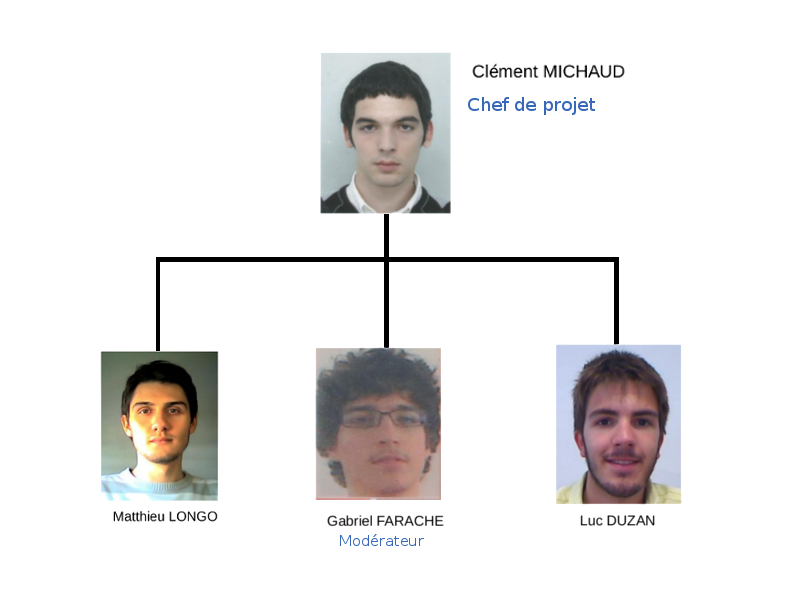
\includegraphics[scale=0.4]{hierarchie.png}
\caption{Hiérarchie de l'équipe}
\label{hierarchie-equipe}
\end{figure}

Ce dernier a été désigné chef de projet par les membres de l'équipe à la fin de la rédaction du projet documentaire. Puis à la suite d'un cours de Conduite de Projet donné par M. HAMADOUCHE, Gabriel FARACHE a été choisi comme modérateur de l'équipe.\\
La recherche documentaire précédent le démarrage du projet a permis de fixer strictement les spécifications techniques et les limites du projet. Le projet a été facile à partitionner grâce à l'existence de trois grands axes de développement parallèles. Cette configuration de projet a permis à l'équipe de créer trois groupes de travail indépendants. Un premier sur du développement logiciel, un deuxième sur du développement matériel en Verilog et un troisième de deux élèves sur la reconfiguration à chaud.\\
Une telle configuration a pu être appliquée au début du développement mais a vite été limitée à cause de la difficulté du sujet. Par la suite, dû aux nombreuses problématiques qui se sont posées, une attitude \textbf{Agile} a été adoptée. Des membres de l'équipe ont été réquisitionnés pour travailler sur un point ou une problématique précise. Cela a permis au groupe de traiter rapidement et efficacement des besoins essentiels nécessaires à l'avancement du reste du projet.

\section{Espace communautaire}

Le projet, c'est-à-dire, les documents écrits, les codes sources, les outils ou autres documentations ont été partagés entre tous les membres de l'équipe grâce un outil de \english{versionning} appelé Git sur un serveur en ligne hébergé par \href{https://github.com}{GitHub}. Cela a permis d'avoir des versions toujours à jour des fichiers que chacun modifie et a surtout été utile pour la gestion du code source composé de nombreux fichiers.\\
L'espace de stockage est largement suffisant pour stocker tous les documents du projet et s'échanger des fichiers si l'envoi de mail ne suffit pas. Le quota de stockage sur Github est de 1GB.\\
Le \english{versionning} dans un projet où le code source est abondant a l'avantage d'autoriser la restauration de versions antérieures du projet qui fonctionnent. Il est également possible de créer des branches de développement indépendantes fusionnables lorsque le développement est terminé.

\section{Communication intra-équipe}
Pour communiquer, les membres de l'équipe ainsi que les tuteurs ont utilisé principalement l'email, moyen efficace et rapide qui permet de transmettre du texte comme des données (dans une limite raisonnable) instantanément.\\
L'un des points forts de notre management de projet a été le nombre de réunions qui ont été organisées. Cela pouvait aller de une à deux par semaine dans lesquelles nous discutions de l'avancement des tâches entreprises et d'une réassignation des tâches jusqu'à la réunion suivante. Un diagramme de Gantt et un tableau des restes à faire proposés par M. HAMADOUCHE, ont été mis en place pour suivre pas à pas l'évolution du projet.

\newpage

\chapter{Contexte du sujet}
\section{Les puces \fpgas{} ou \english{Field-Programmable Gate Array}}

Les \fpgas{} (\english{Field-Programmable Gate Array}) sont des puces qui contiennent un réseau reconfigurable de logique. Les puces peuvent être configurées pour réaliser n'importe quelle fonction logique complexe comme un processeur par exemple. Il existe plusieurs constructeurs de \fpgas{}, les deux plus connus sont \brand{Xilinx} et \brand{Altera}. La configuration d'un \fpga{} est obtenue après ce qu'on appelle la synthèse d'un code écrit en langage HDL (\english{Hardware Description Language}) et le routage des liens entre les différentes logiques. Le fichier généré s'appelle un \english{bitstream}. Ces langages sont bien différents des langages de programmation informatique puisqu'ils permettent de décrire un fonctionnement et ne correspondent pas à un algorithme. Ce type de langage permet de faire de la conception \english{hardware} à moindre coût puisqu'on peut réutiliser le même \fpga{} pour plusieurs conceptions. Le code HDL pourra ensuite être utilisé pour graver directement des puces ASIC (\english{Application-Specific Integrated Circuit}) et obtenir un produit fini.\\

Les \fpgas{} sont constitués d'un nombre très importants de blocs logiques organisés en matrices (d'où le terme \english{Array} dans \fpga{}). Ces blocs logiques élémentaires (AND, OR, XOR, NOT) peuvent être configurés pour effectuer d'autres fonctions logiques bien plus complexes. Il est aussi possible d'utiliser des bascules ou d'autres éléments permettant de mémoriser de l'information. Les nouveaux \fpgas{} contiennent des blocs de RAM de plusieurs kilo octets. Grâce au code HDL, un réseau est tissé et relie toute cette logique pour former un système complexe correspondant à la fonction attendue.\\

De nos jours, les transistors dans les \fpgas{} se comptent en millions. Les puces \fpga{} ne sont en général qu'une partie d'un système plus général. Elles sont implantés sur des circuits imprimés et sont reliées à d'autres périphériques externes comme de la mémoire RAM ou flash, un GPIO (\english{General Purpose Input/Output}), une carte audio, une carte Ethernet. Dans ce projet, nous utilisons une carte de développement appelée \nexys{} développée par l'entreprise \brand{Digilent} qui comprend entre autre une puce \fpga{} Xilinx Spartan 6, un bloc de mémoire RAM et Flash, des LEDS, des boutons, un port Ethernet, un port VGA pour l'affichage sur un moniteur et un port USB.

\section{Les langages HDL}

\subsection{VHDL et Verilog}

Verilog et VHDL (pour \english{Very High speed integrated circuit Hardware Description Language}) sont les deux langages de description de matériel (en anglais, \english{Hardware Description Language}) les plus connus. Ils ressemblent respectivement au langage \languagetoto{ADA} et \languagetoto{C}. Les HDL utilisent une méthode de description de flux de processus résultant d'un modèle de flux de données avec des informations de synchronisation. Cette méthode consiste en une abstraction au niveau des portes logiques et des transitors. Cette méthode s'appelle \english{Register-Transfer Level} (RTL) et a été définie à cause de l'explosion de la complexité des circuits électroniques depuis les années 1970 (loi de Moore). Ce niveau génère ce qu'on appelle une \english{netlist}. Les concepteurs de matériel micro-électronique avaient besoin d'une méthode de description logique des matériels numériques de plus haut niveau pour limiter la complexité de la conception et cela sans que cette dernière ne soit spécifique à une technologie en particulier. À partir de cette représentation des circuits, des représentations de plus bas niveaux et le câblage sur une carte donnée peuvent être déduits. Une \english{netlist} est indépendante de la plateforme tandis qu'un routage lui l'est.\\

Les HDL permettent de décrire un circuit électronique tant au niveau comportemental que structurel, c'est-à-dire les flux de signaux transitant entre les différents registres. C'est pour cette simplification dans la conception et l'utilisation des matériels que les HDL sont largement utilisés dans l'industrie.\\
\begin{figure}[h!]
\centering
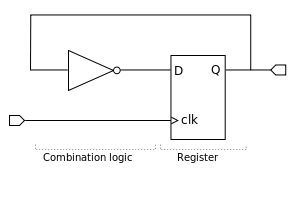
\includegraphics[scale=0.9]{rtl_example.png}
\caption{Bascule D}
\label{BasculeD}
\end{figure}
La figure \ref{BasculeD} montre comment est représenté un circuit. Nous constatons qu'il est ici totalement fait abstraction de la manière avec laquelle ce dernier est câblé. Nous ne connaissons que ce qui est en entrée et sortie de ce dernier. Un HDL décrira, quant à lui, le {\og}comportement{\fg} externe, général du circuit.\\
L'une des principales différences entre les HDL et les langages de programmations traditionnels est qu'avec un HDL il est possible de modéliser plusieurs processus parallèles. Par exemple, un changement dans un des processus pourra donc déclencher une mise à jour dans les autres processus.\\
\\
VHDL et Verilog ont chacun leurs atouts listés non exhaustivement ici :
\begin{itemize}
\item VHDL :
    \begin{itemize}
    \item ce langage a été conçu pour aider la conception et la spécification au niveau d'un système électronique,
    \item il est plus souple que Verilog car permet, entre autre, à l'utilisateur de définir ses types, ses configurations, etc.
    \end{itemize}
    \vspace{10px}
    \item Verilog :
    \begin{itemize}
    \item conçu de base pour les concepteurs de matériel développant des \fpgas{} et ASICs
    \item parfait pour convertir des types de données de vecteurs de bits vers des notations arithmétiques,
    \item existence de supports compréhensibles pour la conception numérique de bas niveau.
    \end{itemize}
\end{itemize}
\vspace{10px}
VHDL et Verilog sont tous les deux des standards IEEE : \textit{IEEE standard 1076-1987}
\cite{IEEE_VHDL_87}
en 1987 puis \textit{IEEE standard 1076-1993}
\cite{IEEE_VHDL_93}
 en 1993 après une mise à jour pour VHDL. Il a ensuite été mis à jour régulièrement pour arriver, en 2008 au standard \textit{IEEE 1076}
\cite{IEEE_VHDL}
 (VHDL 4.0) qui est la dernière version en date. Quant à Verilog, il est devenu un standard en 1995 : \textit{IEEE standard 1364-1995}
\cite{IEEE_VERILOG_1995}
et a été mis à jour deux fois depuis : en 2001 \textit{IEEE Standard 1364-2001}
\cite{IEEE_VERILOG_2001}
(Verilog 2001) qui corrigera de nombreux problèmes puis en 2005 \textit{IEEE Standard 1364-2005}
\cite{IEEE_VERILOG_2005}
(Verilog 2005) qui corrigea quelques bogues.\\

Historiquement, VHDL a été développé pour l'armée de l'air des États-Unis d'Amérique (contrat \textit{F33615-83-C-1003}) par \brand{Intermetrics, Inc.}, \brand{Texas Instruments} et \brand{IBM}. \brand{Intermetrics, Inc.} fournissait les experts en langage de programmation et était aussi le maître d'\oe{}uvre du projet. \brand{Texas Instruments} se concentrait sur la partie expertise en conception de puces. \brand{IBM} quant à elle fournissait les experts en conception de systèmes informatiques. C'était donc un projet de envergure (comme \languagetoto{ADA} par exemple). Verilog a quant à lui été démarré en 1984 par \brand{Gateway Design Automation Inc.} puis rendu disponible au grand public en 1990 par \brand{Cadence}.

\subsection{Les autres langages HDL existants}

Il existe bien d'autres langages que Verilog et VHDL. Altera HDL (AHDL) est un langage propriétaire d'\brand{Altera}, Hydra est fondé sur \languagetoto{Haskell}, MyHDL est fondé sur \languagetoto{Python} ou encore RHDL qui s'appuie sur \languagetoto{Ruby}. Un autre langage appelé \languagetoto{SystemC} est très utilisé dans l'industrie. Cependant, ce dernier n'est pas un langage à part entière puisqu'il utilise un ensemble de classes \languagetoto{C++} fournissant les outils nécessaires à la modélisation du matériel. 


\section{Le système embarqué OpenSource \textit{Milkymist}}

\subsection{Généralités}

\textit{Milkymist} est un système embarqué (\english{System-on-Chip}) développé par plusieurs personnes et entreprises qui permet un traitement d'image vidéo et de son en temps réel.\\
Ce projet a pour origine le projet de fin d'étude du français Sébastien Bourdeauducq \cite{BOURDEAUDUCQ} sur le design d'un système embarqué au \english{Royal Institute of Technology} de Stockholm en 2010. Plus précisément, il s'agissait de réaliser un système rapide et économe en ressources qui utilisait un \fpga{} et avec pour but principal de supporter une application de rendu d'effets vidéo et audio en temps réel. Ce système est totalement indépendant et peu emcombrant.\\
La différence par rapport au traitement d'un ordinateur classique est que cette plateforme \textit{Milkymist} est dédiée à cette tâche et la carte est pourvue de toutes les connectiques nécessaires pour effectuer sa tâche. Le système d'exploitation qui s'exécute est lui plus léger qu'un système d'ordinateur, il permettra donc d'utiliser au mieux la puissance du processeur et des périphériques.

\subsection{Aspects techniques}


\subsubsection{Le matériel}

La carte, appelée \textit{Milkymist One}, est dotée d'une puce \fpga{} sur laquelle on trouvera notament un processeur LatticeMico32 (LM32)\cite{LATTICE}, différents composants de pilotage des périphériques externes (RAM, Flash, etc), plusieurs contrôleurs de bus. Ce processeur est un CPU (\english{Central Processing Unit}) 32-bit \english{big endian} RISC OpenSource développé par \brand{Lattice Semiconducteur}. Il suit une architecture Harvard. Ce microprocesseur est assisté dans son travail par une unité de mappage de texture et par un coprocesseur programmable à virgule flottante qui est utilisé par le logiciel de synthèse video.\\

Sur la carte, représentée par la figure \ref{milky-board}, se trouve différents périphériques. On y trouve de la mémoire RAM et Flash, un contrôleur de communication série (UART pour \english{Universal Asynchronous Receiver Transmitter}), des ports USB, un port Ethernet et un lecteur de cartes SD.
La carte a pour vocation primaire de faire du traitement multimédia tant audio que vidéo, c'est pourquoi la carte dispose également des périphériques orientés multimédia tels qu'une carte son avec prise jack, une sortie VGA pour afficher la vidéo, un port MIDI pour brancher des instruments par exemple, un récepteur IR et une entrée vidéo PAL/NTSC. Notons que \textit{Milkymist} possède aussi son propre langage HDL appelé \languagetoto{Migen} qui est toujours en développement.

\begin{figure}[h!]
\centering
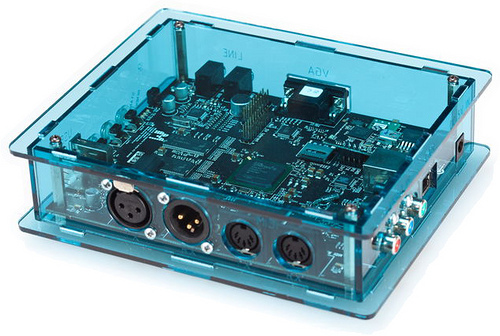
\includegraphics[scale=1]{milky_board.jpg}
\caption{Photo de la Milkymist One}
\label{milky-board}
\end{figure}

\subsubsection{Le firmware}

Le système d'exploitation qui s'exécute sur la \textit{Milkymist One} est une distribution linux appelée \textit{uClinux} qui a été adapté en même temps que la carte. Cette version de linux fonctionne sur des processeurs dédiés aux systèmes temps réel, c'est-à-dire des systèmes qui n'ont pas de MMU (\english{Memory Management Unit}) et qui ne gère pas de mécanismes de protection de la mémoire. Ce système d'exploitation a déjà été porté sur des microcontrôleurs comme certains 8-bits fabriqués par \brand{Atmel} ou d'autres PIC de chez \brand{Microchip}.\\
Le système complet se compose d'un BIOS écrit en ROM qui charge le noyau par le biais d'internet ou de la carte SD et de toutes les applications de traitement multimédia.\\

La carte dont dispose l'INSA, la \brand{Digilent} \nexys{} (figure \ref{nexys3-board}), comprend également une Spartan6 ainsi qu'un bloc de 16 MB de RAM, une interface de sortie VGA, un connecteur USB et un port Ethernet.

\begin{figure}[h!]
\centering
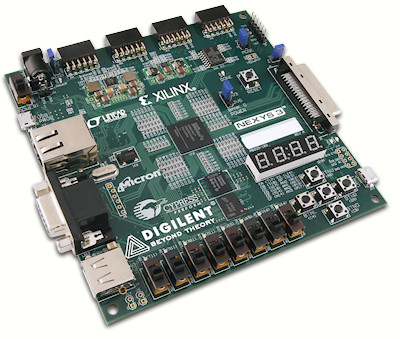
\includegraphics[scale=0.5]{nexys3.jpg}
\caption{Photo de la \nexys{} distribuée par \brand{Digilent}}
\label{nexys3-board}
\end{figure}


\newpage


%%%%%%%%%

\chapter{Adaptation d'un système embarqué libre : \textit{Milkymist}}

\section{Adaptation du système}

Lorsque l'on veut adapter un système existant qui fonctionne sur une machine pour le faire fonctionner sur une autre machine, on dit qu'on \textbf{porte} un système. C'est ce qui a été envisagé dans ce projet.\\
\textit{Milkymist} est un système dont le code HDL et le code \languagetoto{C} du système d'exploitation sont totalement OpenSource et donc réutilisables et modifiables.\\
L'INSA dispose de cartes de développement \nexys. Cette carte ressemble à une \textit{Milkymist One} car elles sont toutes les deux dotées d'une puce \fpga{} Spartan6 et ont des périphériques communs tels que la mémoire et l'UART.\\

Le projet consiste donc au portage de l'architecture (figure \ref{milky-archi}) et du système logiciel \textit{Milkymist} en laissant de côté le multimédia pour avoir un système embarqué fonctionnel sur la \nexys qui permettrait par la suite de tester la technologie récente appelée \english{partial reconfiguration} par \brand{Xilinx} et dont l'abréviation est \textbf{PR}.

\begin{figure}[h!]
\centering
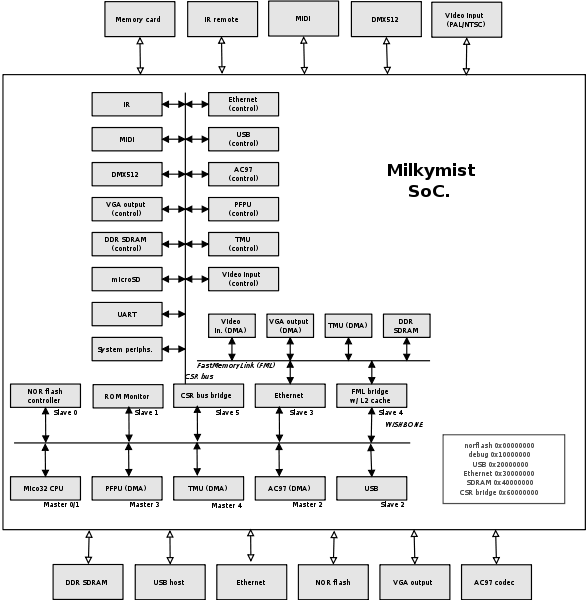
\includegraphics[scale=0.7]{milky_archi.png}
\caption{Architecture du système Milkymist}
\label{milky-archi}
\end{figure}

\subsection{La simulation sous Qemu}

Le but de cette partie était d'adapter le noyau linux (uClinux) de \textit{Milkymist} en se basant sur le portage réalisé par \brand{Theobroma-Systems}. Il nous fallait aussi créer un système de fichier minimal associé à ce noyau. Nous avons rencontré de problèmes liés aux outils de compilations. Ces bugs liés aux outils de compilations ont été corrigés. Une fois ce correctif appliqué, nous avons créé le système de fichier à l'aide d'\textit{OpenWrt}, qui a pour but de simplifier l'utilisation de linux sur différentes platforme, dont la carte de \textit{Milkymist}.\\
La création d'un noyau et d'un système de fichiers a donc été un succès et cela malgré le temps passé à bloquer à cause d'erreurs dans les outils de compilation.

\subsection{Le système sur cible réelle}

Dans un second temps, il nous fallait démarrer le noyau sur la \nexys{}. Nous avons dû modifier le code source du BIOS fourni par \textit{Milkymist} pour pouvoir démarrer le noyau présent en mémoire Flash. Le noyau est chargé via un outil JTAG développé par nos soins. Le BIOS doit ensuite le démarrer.\\

Nous avons rencontrés des problèmes lors du débogage du noyau à cause d'erreurs rendant l'affichage inopérant cela nous empêchant de détecter précisément leurs causes. De même, la modification du BIOS a été d'autant plus complexe que nous ne l'avions pas écrit. En effet, nous nous contentions de commenter ou de décommenter du code. Cependant, nous avons pu vérifier le bon fonctionnement des procédures de démarrage du noyau et en déduire que les erreurs se situaient à sa compilation. 



\section{Tests du matériel}

\subsection{La PSRAM}

Suite à des problèmes d'exécution du bios puis de démarrage de uClinux, nous avons tout d'abord voulu regarder si le contenu de la RAM était correct. Pour cela, nous souhaitions faire une simulation globale du système et regarder le contenu de la RAM. Or sur la \nexys{}, la RAM est un périphérique externe et n'a donc pas de relation avec le code HDL, elle est seulement connecté au reste par un contrôleur en Verilog. La première étape a consisté au remplacement de ce module par un module appelé BRAM codé en Verilog (RAM réalisé en portes logiques dans le FPGA) qui allait pouvoir être simulé.\\
Une fois cette tâche réalisée, nous avons voulu vérifier qu'il ne s'agissait pas d'un problème de communication avec le bus et que les signaux étaient corrects. Le problème pouvait également venir du module multiplexeur qui permet de sélectionner la mémoire soit flash soit RAM car leur bus de données est partagé.

\subsection{Simulation du système complet}

Cette simulation ne s'est pas révélée si aisée qu'on le pensait. Le système a une taille considérable et simuler seulement 0.2s nécessitait plusieurs minutes et une cinquantaine de gigaoctets. Finalement, après de multiples problèmes de compilation après modifications du testbench original, nous avons préféré abandonner. Comme le montre le schéma à la figure \ref{milky-archi}, l'architecture comprend trois bus différents, ce qui n'était pas du tout justifié pour notre projet et compliquait énormément notre tâche. Le bus Wishbone aurait seul suffit.

\section{La \english{Partial Reconfiguration} (PR)}

\subsection{Généralités}

La \english{partial reconfiguration} est un concept qui existait déjà dans les années 70 mais qui a vu le jour en 2009 lorsque les fabricants de puces \fpgas ont pris conscience des possibilités immenses de cette technologie. C'est l'arrivée des \fpgas{} qui a permis d'aboutir au développement de la \english{partial reconfiguration}.\\
Elle consiste à appliquer le procédé de reconfiguration sur une petite partie du \fpga{} en laissant fonctionner normalement la partie qui n'est pas reconfigurée. On parle aussi de reconfiguration à chaud, c'est-à-dire que le système n'est pas entièrement éteint lorsque l'opération est exécutée. Cela permet alors dans le cas d'un \english{System-On-Chip} de rajouter dynamiquement des modules sans devoir redémarrer le système. On peut alors concevoir un grand nombres de modules spécifiquement optimisés pour certaines applications (cryptologie, calcul flottants) pour lequel l'architecture initiale du processeur est peu optimale. Grâce au PR, la taille du \fpga{} n'est plus limitante puisque l'on peut implanter n'importe quel module. Cela permet de multiplexer temporellement les ressources du \fpga{} et d'économiser de l'énergie en enlevant des modules non utilisés.

\subsection{Les différents types de \english{partial reconfiguration}}

Il existe deux grands types de reconfigurations pour les \fpgas{} de \brand{Xilinx}. Il existe deux méthodes : \english{difference-based} et \english{module-based}.\\

La reconfiguration \english{difference-based} existait avant la \english{module-based}. La deuxième est un cas particulier de la première. La reconfiguration \english{difference-based} consiste à générer ce qu'on appelle un \english{partial bitstream} qui ne représentera que la différence d'une configuration initiale avec cette nouvelle configuration. Cette méthode est illustrée à la figure~\ref{partial-bitstream}. À partir de la configuration initiale et de ce \english{partial bitstream}, on obtient la deuxième configuration. Une option dans les outils de synthèse \brand{Xilinx} permet de générer un \english{bitstream} qui est la différence entre le premier système et le second. Le \fpga{} ne reconfigurera que les parties différentes.\\
\begin{figure}[h!]
\centering
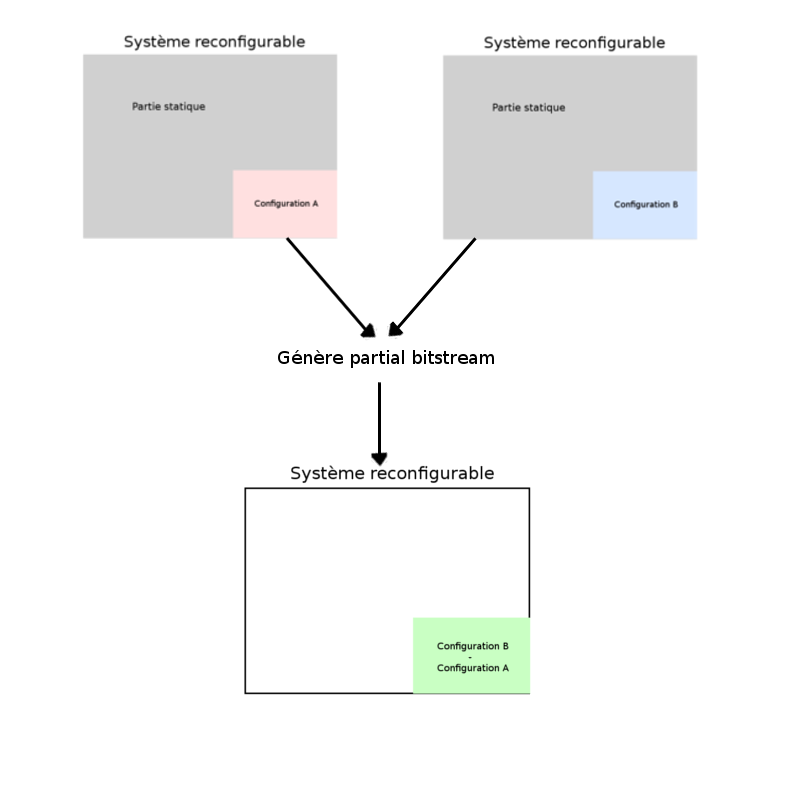
\includegraphics[scale=0.4]{pr2.png}
\caption{Génération d'un \english{partial bitstream}}
\label{partial-bitstream}
\end{figure}
Cette solution est adaptée pour des reconfigurations de petite envergure, mais assez peu efficace pour une solution plus complexe telle qu'envisagée dans le projet. En effet, la taille du \english{bitstream} grossit en fonction de la différence entre les deux circuits. Le but de notre projet est de pouvoir configurer à chaud un module appartenant à une \english{library} à développer.\\

La deuxième technique est la \english{partial reconfiguration module-based} qui consiste à segmenter le \fpga{} en zones. Il est ensuite possible d'instancier un module Verilog dans une zone. On appelle ces zones des tranches (\english{slices} en anglais). Il peut y avoir plusieurs tranches dans un projet mais il n'est possible d'allouer qu'un module par tranche à la fois. La reconfiguration s'effectue sur les tranches. Lors d'une reconfiguration, on assigne un module à une tranche, on dit qu'on l'instancie.\\
Considérons une carte mère qui contient des emplacements libres. Un qui peut contenir différents processeurs, un autre différentes cartes graphiques et un dernier qui peut contenir différentes cartes son. Ces emplacements représentent les tranches. Chaque composant représente un module qui peut être instancié dans son emplacement prévu.\\
Finalement, une configuration est une combinaison d'instances, chacune se trouvant dans une tranche. Une configuration est donc un triplet (processeur, carte graphique, carte son). Si le projet comporte trois tranches et trois modules instanciables par tranche alors le nombre de configurations possibles sera de $3^3=27$. Un module peut être instancié dans une tranche et pas dans une autre.\\
Le design doit au moins comporter une tranche dite statique, qui elle, ne peut être reconfigurée. La connexion entre les tranches statiques et les tranches reconfigurables est définie par des pins qui se situent à leurs frontières. Au moment de la conception, on choisit pour chaque tranche le nombre de \english{pins} qu'elle possède et leurs directions (ils ne peuvent être bidirectionel). Les \english{pins} reprèsentent la liaison entre la partie statique et la reconfigurable.\\

Cette méthode n'est pas compatible avec tous les \fpgas{} puisqu'il faut optimiser le routage entre les tranches et cette opération dépend de la plateforme utilisée. ISE, l'outil de gestion de projet et de synthèse de \brand{Xilinx}, ne le supporte pas pour la Spartan6.\\
Le projet étant complexe, la solution du \english{difference-based} ne convient pas.

\subsection{PlanAhead et l'incompatibilité avec la Spartan6}

Le logiciel PlanAhead de \brand{Xilinx} permet de définir les contraintes de routage et de placement des portes logiques d'un module afin qu'il puisse s'adapter à une tranche. Ces tranches sont aussi définies avec ce même logiciel, qui permet ensuite de générer les \english{bitstreams} correspondant à une configuration donnée. Malheureusement, PlanAhead ne permet pas de faire de \english{partial reconfiguration} sur Spartan6. En revanche, il permet de le faire uniquement sur les \fpgas{} suivants : Virtex-4, Virtex-5, Virtex-6, Virtex-7, Kintex-7, Artix-7 et Zynq.\\

Ayant fait une telle découverte, nous avons espéré utiliser la méthode \english{difference-based} pour simuler la méthode \english{module-based} en définissant clairement où se situent les différentes parties statiques et dynamiques. La partie statique étant fixée, il est possible en faisant la différence de deux configurations de faire disparaitre cette partie du \english{partial bitstream} puisqu'elle s'annule. L'inconvénient est qu'il faut alors générer un bitstream pour chaque configuration. Une pour passer d'une configuration $C_{1}$ à $C_{2}$, une de $C_{2}$ à $C_{3}$, une de $C_{1}$ à $C_{3}$ et leurs inverses. L'idée était alors de définir une configuration initiale appelée \english{blank} à partir de laquelle il est possible de se rendre dans n'importe quelle configuration et ensuite d'y revenir. Ainsi il est possible de réduire à deux le nombre de \english{partial bitstreams} à générer. Le fichier pour se rendre de Blank à $C_{x}$ et un fichier de $C_{x}$ à Blank.


\section{Bilan technique}
\subsection{Quelques difficultés}

Le projet MilkyMist s'est révélé être trop important et complexe pour être pris en main de manière rapide et efficace. La partie hardware contenait beaucoup de modules inutiles et le design du système en lui-même n'était pas très adapté à notre utilisation. Il était difficile d'éviter les effets de bords lorsqu'on supprimait un module. La simulation du système était une tâche dont l'ampleur avait été sous-estimée.\\
Nous avons également été confronté à des problèmes au niveau du système qui ne démarre pas sur la \nexys{}. Plusieurs pistes ont été explorées mais aucune n'a porté ses fruits. Le travail a été d'autant plus compliqué que nous ne possédions pas un système complet et fonctionnel (nous n'avions pas de RAM). Une dernière piste possible, non explorée à ce jour par manque de temps, est le \english{Device Tree Source} ou \textit{DTS}. Ce fichier permet au noyau de connaître ses périphériques mais puisque nous ne travaillons pas sur la même carte que celle de MilkyMist, les périphériques ne sont pas les mêmes et les adresses où ils se trouvent sont différentes. Ce problème est d'autant plus ennuyant que sur cible simulée, le noyau et son système de fichier fonctionnent parfaitement.\\
Le temps d'installation de tous les outils sur les machines est très long à cause notamment des bugs de version. La compilation du compilateur pour LM32, l'installation de ISE, les problèmes de bibliothèques manquantes ont aussi été problématiques. Les différentes versions de linux utilisées ont posé des problèmes de compatibilités qui ont obligé certains membres de l'équipe à créer une \english{sandbox} afin d'exécuter des programmes compilés sur d'autres machines.

\subsection{Réorientation vers une nouvelle solution \english{from scratch}}

Le système \textit{Milkymist} est un système complexe et il a paru plus facile d'en recréer un avec les modules nécessaires mais en partant de zéro. Tout refaire depuis le début nous a donné l'avantage d'avoir une meilleure maîtrise du code. Il en a été de même pour le software puisqu'il a été décidé de créer notre propre kernel.

\newpage


\chapter{Vers un nouveau SoC}

\section{Réalisations matérielles}
\subsection{Architecture du nouveau système}

La solution de création d'un nouveau SoC est une solution qui paraissait réaliste. Un projet avait déjà été commencé par \textit{G33KatWork} sur \href{https://github.com}{GitHub}. Ce projet était le début d'un système pour plusieurs plateformes dont la \nexys{}. Le projet comportait déjà un coeur LatticeMico32, de la RAM, un contrôleur UART, deux timers, un GPIO, le tout interfacé en Wishbone grâce à un connecteur \textit{Conbus} adapté, visible dans la figure \ref{new-system}.\\
Ceci a donc fourni la partie hardware minimale pour travailler mais aucun système logiciel ne l'accompagnait. Il fallait alors développer un firmware qui le ferait fonctionner.

\begin{figure}[h!]
\centering
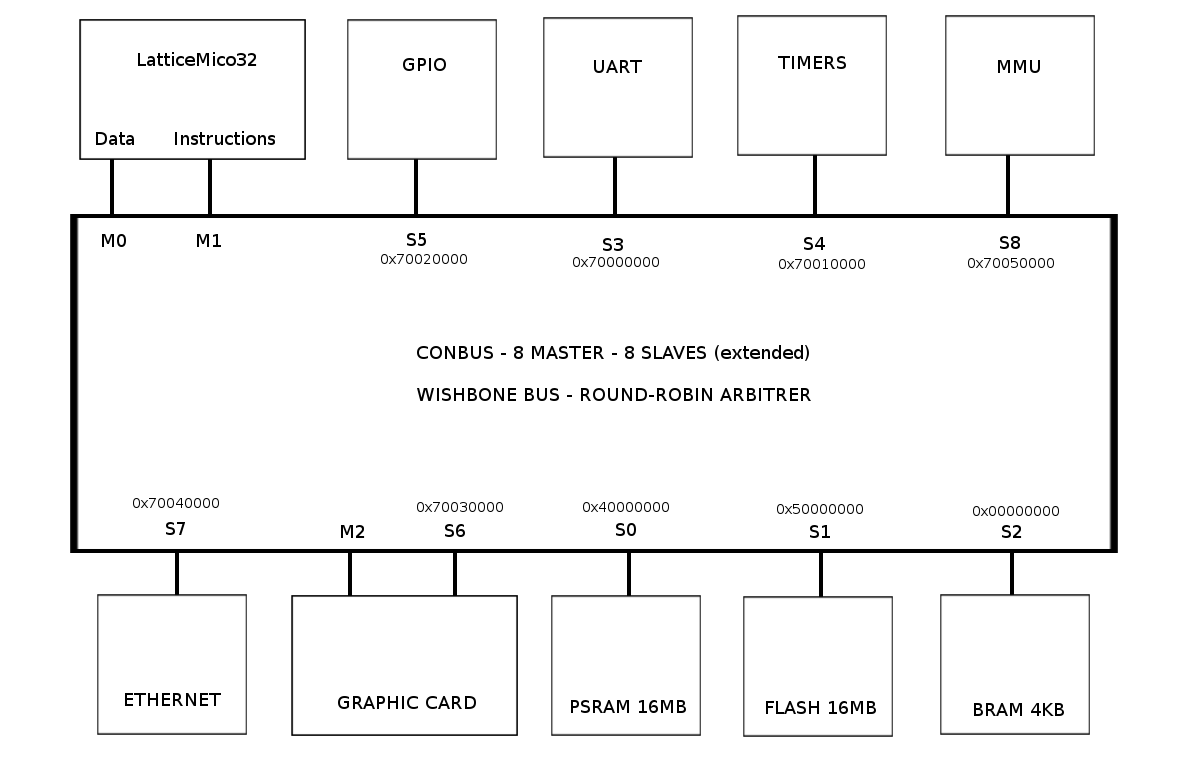
\includegraphics[scale=0.35]{general_system.png}
\caption{Schéma de l'architecture du nouveau système}
\label{new-system}
\end{figure}

\subsection{Le \english{bootloader}}

La premier programme réalisé a été le \english{bootloader} qui permet de charger en RAM un code par le biais de l'UART. Ce \english{bootloader} est implanté directement dans une RAM de 4096 octets réalisée en HDL. Le code du \english{bootloader} ne compte que quelques octets une fois compilé et s'exécute à chaque \english{reset} du processeur.\\
Ce logiciel, développé en \languagetoto{C} et appelé INSAFirmware, accueille l'utilisateur et se met en attente d'un fichier sur l'UART.\\
L'utilisateur doit alors envoyé 4 octets représentants la taille du fichier à lire par l'UART, les 4 octets suivant permettent de définir l'adresse où sera stocké le fichier. En général, ce code sera stocké en RAM. Finalement, l'utilisateur peut commencer à envoyer octet par octet son programme. Une fois le programme chargé, le firmware saute à l'adresse fournie par l'utilisateur et commence à exécuter le code.

\subsection{Création de nouveaux modules}

\subsubsection{Module Flash}

Pour compléter le système, le code Verilog du contrôleur de mémoire flash de \textit{Milkymist} a été récupéré et adapté sur le nouveau système. Il a ensuite fallu créer un driver qui permet de lire et d'écrire dans cette mémoire non volatile car son interface de contrôle fonctionne par commandes. Il faut écrire un octet de commande pour que la mémoire effectue la commande associée.\\
Il est actuellement possible d'écrire et lire des mots de 16 bits.

\subsubsection{Carte graphique}

La création d'une carte graphique a été entreprise. Elle comprend la gestion de la mémoire vidéo et l'affichage sur un moniteur connecté en VGA. Le schéma général de la carte graphique est présenté en figure \ref{carte-graphique}.

\begin{figure}[h!]
\centering
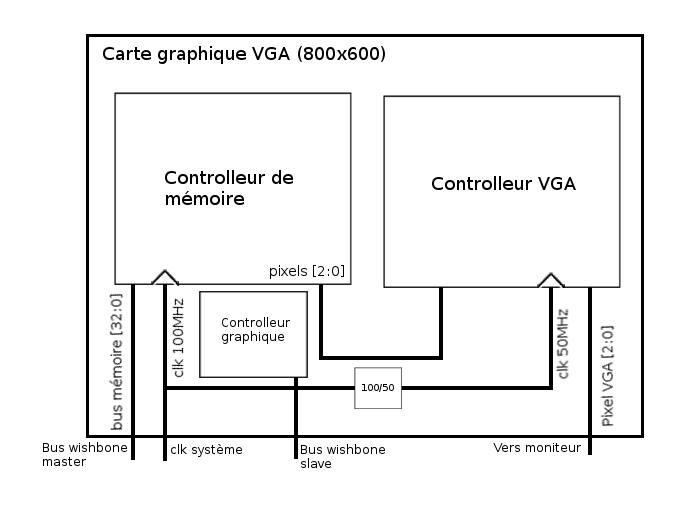
\includegraphics[scale=0.5]{vga.png}
\caption{Schéma de la carte graphique}
\label{carte-graphique}
\end{figure}

Cette carte graphique est reliée au bus Wishbone en tant qu'esclave grâce au contrôleur graphique qui permet de sélectionner l'adresse de base de la mémoire vidéo et d'activer ou de désactiver la carte graphique.\\
L'interface Wishbone maître sert à envoyer les requêtes mémoire pour acquérir les pixels du moniteur. De cette façon le contrôleur de mémoire s'exécute en parallèle du processeur. Il n'y aura pas d'accès mémoire concurrents puisque le \textit{Conbus} suit une stratégie \english{round-robin} pour la prise du bus.\\

Le contrôleur VGA actuellement implémenté dans la carte, ne permet d'afficher qu'une résolution de 800x600 mais pourrait facilement être modifié pour rendre possible le paramétrage dynamique de la résolution. Ainsi, on pourrait changer la résolution au niveau logiciel.\\
L'une des grandes problématiques est que la RAM embarquée sur la \nexys{} n'est pas assez rapide pour être lue à la fréquence de rafraichissement de l'écran. Il a donc fallu implémenter un système de bufferisation dans le contrôleur de mémoire. Celui-ci affiche $N$ pixels puis utilise les $3*N$ pixels suivant pour bufferiser les $N$ pixels qui suivront. On divise ainsi la fréquence d'affichage par quatre mais on obtient un affichage complet de l'écran. Cette manière de procéder fonctionne aussi pour des résolutions différentes.\\

À l'heure actuelle, la carte graphique n'est pas fonctionnelle mais est en bonne voie pour le devenir. La RAM de la \nexys{} fournit un moyen de lire un mot de 16 bits à chaque \english{tick} d'horloge système (100MHz) pendant 16 \english{ticks}. C'est ce qu'on appelle un \english{page mode}. On lit plusieurs valeurs à la suite sans attendre le temps de rafraîchissement de cette valeur comme dans un \english{single-read mode} où une seule valeur est lue à la fois. Cette fonctionnalité est en train d'être ajoutée au niveau matériel au contrôleur de PSRAM afin de gérer ce mode et ainsi d'accélérer la bufferisation pour essayer de passer à un taux de rafraîchissement seulement divisé par deux.\\

Il n'existe sur la \nexys{} qu'une mémoire capable d'être lue à la volée à la fréquence demandée : la flash avec interface SPI en \english{quad mode}. SPI est un protocole créé par des entreprises pour effectuer des communications série, c'est-à-dire qu'il ne faut qu'un seul \textit{pin} de données pour communiquer avec le périphérique. Cette flash a en plus un \english{quad mode} qui permet de lire 4 bits à chaque \english{tick} d'horloge, ceci permet de multiplier le débit par quatre. Dans ce mode, la fréquence maximale de fonctionnement est la même que celle du VGA (50MHz). En arrivant à l'interfacer, nous pourrions alors tenter d'afficher des images sans bufferisation mais une mémoire flash est beaucoup plus sensible aux cycles d'écritures et vieillit plus vite qu'une RAM.

\subsubsection{\english{Memory Management Unit}}

Une MMU est un composant qui permet de faire une translation d'adresse entre espace virtuel et espace physique. Cette MMU très simple pourrait permettre d'implémenter un fonctionnement multi-tâches tel qu'il est fait sur les ordinateurs classiques. La translation d'adresses est illustrée dans la figure \ref{memory-management-unit-translation}.

\begin{figure}[h!]
\centering
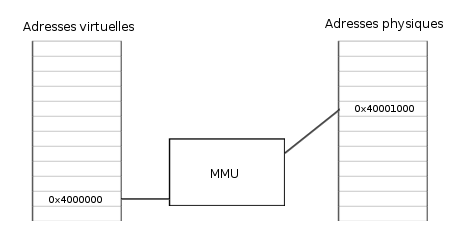
\includegraphics[scale=0.6]{mmu_translation.png}
\caption{Schéma d'une translation d'adresses virtuelles à physiques}
\label{memory-management-unit-translation}
\end{figure}

Ce module Verilog coupe le bus d'adresse du LatticeMico32 pour faire la translation. Il a une interface esclave connectée au bus Wishbone qui lui permet d'être paramétré. Cette MMU est illustrée à la figure \ref{memory-management-unit}.\\
Son fonctionnement est simple, on peut l'activer ou la désactiver en écrivant dans le registre de contrôle. Lorsqu'elle est désactivée, il n'y a pas de translation d'adresse, c'est-à-dire que l'adresse physique est égale à l'adresse virtuelle. Si elle est activée, elle
utilise un deuxième registre qui stocke la valeur de l'\english{offset} à ajouter à l'adresse virtuelle. Ainsi, si l'adresse en entrée (l'adresse virtuelle) est de 0x40000000 et que l'\english{offset} de la MMU est 0x1000, l'adresse physique sera 0x40001000.

\begin{figure}[h!]
\centering
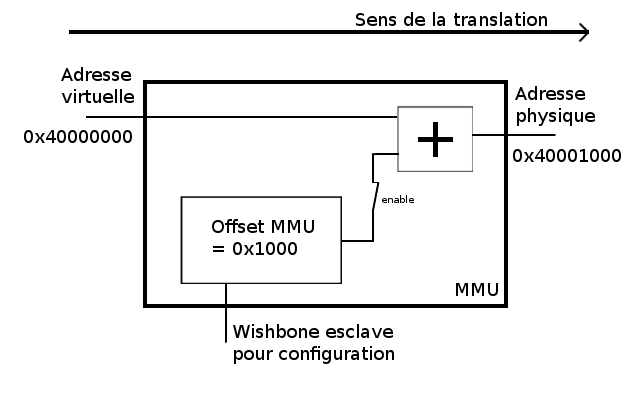
\includegraphics[scale=0.5]{mmu.png}
\caption{Schéma de la MMU}
\label{memory-management-unit}
\end{figure}

\subsubsection{Module Ethernet}

Nous avons trouvé un module Ethernet sur un \href{http://svn.ohwr.org/lm32/cores/mac/rtl/}{SVN}. Il s'agissait du même module que celui proposé sur \href{http://opencores.org/project,ethmac}{OpenCores}. Ce module a une interface de bus Wishbone, il avait été utilisé précédemment dans un système avec un LM32. L'idée est de pouvoir relier deux cartes avec un câble Ethernet et d'utiliser cette interface de communication afin d'échanger des données. Cette interface nous offre des services de base (CRC, accès au medium CSMA/CD) pour envoyer des données de manière à résister à des accès simultanés au medium et des erreurs de transmission dues aux interférences.\\

Nous avons également trouvé le driver de ce module sur le même \href{http://svn.ohwr.org/lm32/crt/mac/}{SVN}. Cependant, pour que ce driver soit fonctionnel, il faudrait connecter l'interruption au processeur, puis gérer l'interruption associée dans le kernel.


\section{Développement d'un noyau minimal}
Après quelques tentatives infructueuses pour porter le noyau linux sur le matériel, la création d'un noyau minimal semblait être un bon compromis car pour utiliser le \textit{PR}, même un noyau basique voire pas de noyau aurait pu suffir.

\subsection{Ses fonctionnalités}

Le noyau qui a été développé en \languagetoto{C++} gère des mécanismes minima. Il permet d'utiliser l'UART pour dialoguer avec l'utilisateur. Un tas a été créé pour permettre l'allocation dynamique de mémoire. Il est possible de paramétrer sa position et sa taille en mémoire.\\
Un driver de VGA a été entrepris mais non terminé puisque le VGA n'est pas tout à fait fonctionnel.\\
Ce noyau gère aussi les interruptions matérielles comme la réception d'un octet sur l'UART et les interruptions des timers.
Un des timers génère une interruption périodique réglable qui pourrait être utilisée pour du \english{multitasking}.\\
Actuellement, aucun appel système n'est géré mais ils peuvent être implémentés aisément.

\subsection{Un pseudo-terminal}

Le pseudo-terminal a été développé en \languagetoto{C} et a pour but de permettre à l'utilisateur de lancer un programme présent en mémoire flash. Le fichier de configuration contient plusieurs lignes associant des informations (adresse en flash et taille) à un programme. Il a aussi pour but de pallier au manque de système de fichiers. En effet, le programme récupère ses informations dans un fichier de configuration présent à une adresse fixe en flash. Lorsque l'utilisateur entre une commande dans le pseudo-terminal, ce dernier va parcourir le fichier de configuration pour trouver les informations associées à la commande entrée par l'utilisateur. Si le nom demandé n'est pas trouvé, une erreur est affichée. Sinon il devra demander au noyau de charger le programme en RAM et de l'exécuter. Cette dernière partie n'a pas été implémentée puisque l'appel système \texttt{malloc} nécessaire pour la comparaison des noms de programme n'a pas été implémenté.

\subsection{Affichage sur la sortie VGA}

Les données à destination de la sortie VGA sont stockées en RAM à une adresse paramétrable. La fréquence de lecture de la mémoire vidéo se fera à la fréquence de rafraîchissement du VGA. Quant à l'écriture, elle ne sera pas périodique et ne surviendra que lors d'une modification de contenu : lorsqu'on tape au clavier, lors d'un affichage de message sur la sortie standard. Il serait possible d'afficher des images au format Bitmap directement sur le SoC en les convertissant au bon format pour être lisible par le VGA.

\begin{figure}[h!]
\centering
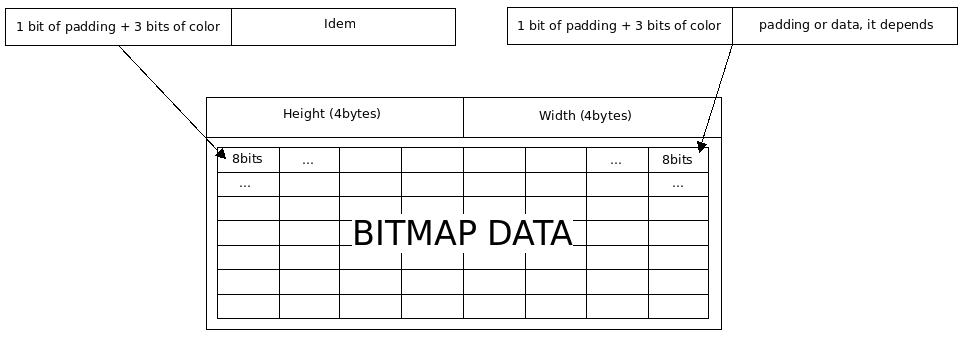
\includegraphics[scale=0.4]{formatBmpFile.png}
\caption{Format du fichier lisible par le VGA}
\label{format-bitmap-vga}
\end{figure}

La mémoire vidéo récupèrera les données du pseudo-format présenté sur la figure \ref{format-bitmap-vga}. La sortie VGA de la \nexys{} ne supporte que 3 bits de couleurs. Nous nous sommes donc contentés de mettre dans l'en-tête du fichier la largeur et la longueur en pixel de l'image, qui sont des informations suffisantes pour déduire par la suite la taille totale de l'image. Cela implique tout de même qu'il faudra faire attention à la taille totale de l'image pour ne pas déborder dans une autre zone de la RAM. Puis s'enchaînent les données dans le format présenté sur la figure \ref{format-bitmap-vga}. Un pixel sera codé sur 3 bits. Il y aura donc 2 pixels par octets et également 2 bits de padding. Il y aura un éventuel padding pour les lignes de pixel pour réaliser un alignement sur 8 bits.

\subsection{Le driver pour l'Ethernet}

Le code du driver a été trouvé comme dit précédemment sur un \href{http://svn.ohwr.org/lm32/crt/mac/}{SVN}. Les parties en assembleur dans le code ne sont pas à réécrire (compatible avec le LM32). Cependant, nous n'avons pas eu le temps de le tester. Il faudrait, pour commencer, regarder les exemples d'utilisation fournis et réaliser un test simple.\\
Plusieurs fonctions tels que \texttt{memcpy}, \texttt{memcmp} ou encore diverses fonctions d'affichage ont été définies pour une autre plateforme. Il faudrait les intégrer à ce qui existe déjà dans notre \english{library} ainsi que le \english{handler} d'interruption.\\
Dans l'état actuel, si on se penche sur les services déjà implémentés, il y a une fonction pour initialiser le module, le désactiver, envoyer et recevoir des données et enfin mettre en place un \english{handler} pour l'interruption associée à la réception de données.



\section{Externalisation du PR}

\subsection{De la \english{partial reconfiguration} sur \virtex{}}

Devant l'impossibilité de faire de la \english{partial reconfiguration} sur Spartan6, une carte de développement dotée d'une \virtex{} nous a été fournie. Ce \fpga{} supporte bien la \english{partial reconfiguration} que ce soit en \english{difference-based} ou \english{module-based}. La solution était alors de garder le système sur la \nexys{} et de la faire communiquer avec la nouvelle carte.

\subsection{Communication entre la \virtex{} et la \nexys{}}

Après avoir examiné les possibilités que nous offraient les deux cartes, nous sommes partis sur l'idée de les faire communiquer via l'interface Ethernet. Évidemment, nous n'avions pas besoin de gérer toutes les fonctionnalités de la \english{link layer} comme définies dans le modèle OSI. Nous recherchions un moyen de communication qui s'occupe de l'accès au medium (CSMA/CD) ainsi qu'une certaine fiabilité des données transmises (CRC).\\
Du côté de la \nexys{}, une couche software s'occuperra de l'émission et de la transmission des données.\\
Sur la \virtex{} (voir figure \ref{virtex5-arch}), il n'y aura que des modules matériels communiquants entre eux :

\begin{itemize}
  \item un module Ethernet pour commmuniquer avec la \nexys{}.
  \item un bus de données Wishbone.
  \item de la RAM afin de stocker les données originales puis les données traitées par le module de PR.
  \item l'ICAP qui permettra de mettre en place le bitstream reçu via Ethernet.
  \item le module de PR qui effectuera les calculs sur les données.
  \item enfin, le module de contrôle du module de PR qui servira d'interface avec le bus et se chargera d'envoyer les données à traiter contenues en RAM vers le module de PR, puis de les récupérer pour les restocker en RAM. Lorsque l'opération sur les données sera finie, il renverra les résultats via l'Ethernet à la \nexys{}.
\end{itemize}

\begin{figure}[h!]
\centering
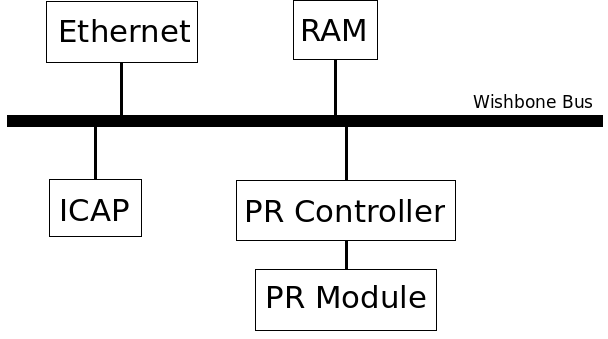
\includegraphics[scale=0.30]{virtex5-arch.png}
\caption{Schéma de l'architecture sur la carte pour le PR}
\label{virtex5-arch}
\end{figure}

\subsubsection{Protocole de communication}

Les échanges de données entre les deux cartes se feront au travers d'un protocole de communication simple. Les actions du côté de la \nexys{} sont illustrées par la figure \ref{nexys-side-protocol} et les actions du côté \virtex{} par la figure \ref{virtex-side-protocol}.\\
Partons de l'hypothèse que la Virtex5 et la \nexys{} sont dans l'état \textit{idle}. La \nexys{} enverra d'abord un ordre de reconfiguration à la Virtex5, puis le bitstream permettant d'effectuer le calcul. Ensuite la Virtex5 sera configurée et renverra un \textit{acknowkedgment} quand elle sera prête. La \nexys{} va alors envoyer les données à traiter puis se mettre en attente du résultat. Du côté de la \virtex{}, le calcul peut alors commencer. Une fois celui-ci fini, le contrôleur du module PR récupérera le résultat dans la RAM puis l'enverra via Ethernet à la \nexys{}.

\begin{figure}[h!]
\centering
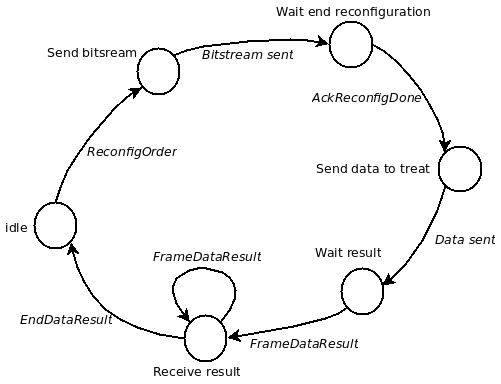
\includegraphics[scale=0.4]{nexys-side-protocol.png}
\caption{Protocole de communication du côté de la \nexys{}}
\label{nexys-side-protocol}
\end{figure}

\begin{figure}[h!]
\centering
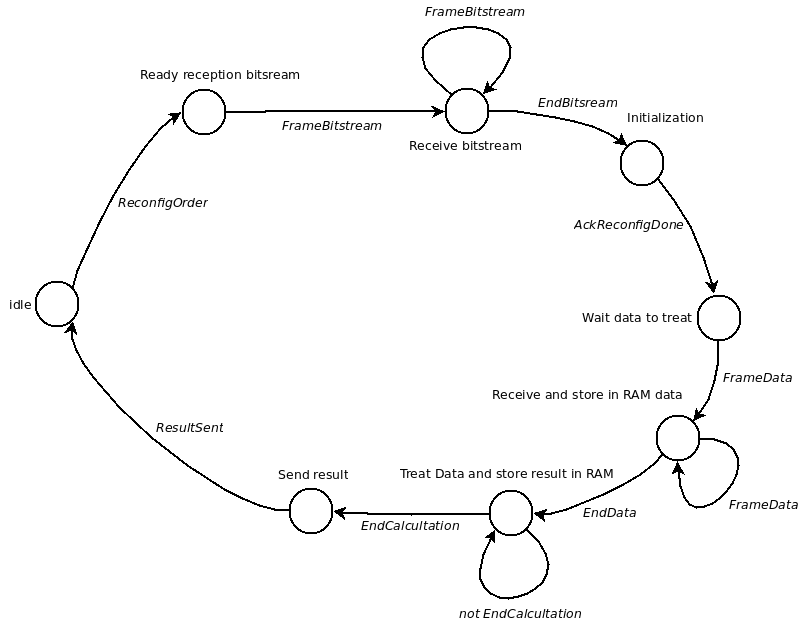
\includegraphics[scale=0.4]{virtex-side-protocol.png}
\caption{Protocole de communication du côté de la \virtex{}}
\label{virtex-side-protocol}
\end{figure}


\newpage



\chapter{Bilan et acquis techniques}

\section{Un projet riche en expériences}
\subsection{En terme technique}

Malgré la difficulté de réalisation de ce projet et le manque de temps pour le développer complétement, les acquis techniques des membres sont conséquents.\\
Ce projet a permis à chacun d'appronfondir grandement sa compréhension des \fpgas{} et leur contenu, c'est-à-dire tout ce que l'on trouve à l'intérieur. On peut citer les \english{logic-blocks}, les \english{I/O blocks}, les blocs de mémoire internes, les arbres d'horloge.\\
La \english{partial reconfiguration} a également permis d'aller plus loin sur la programmation des \fpgas{}, leur configuration interne ainsi que le fonctionnement de la norme JTAG qui permet le débogage du matériel. D'ailleurs, le développement d'un outil JTAG a fortement aidé à sa compréhension.\\

La \english{partial reconfiguration} est une technologie très récente qui a été largement étudiée durant ce projet. Ce savoir pourra tout à fait être réutilisé pour un autre projet ou plus tard dans une entreprise. Les différentes méthodes existantes ont été abordées ainsi que d'autres méthodes développées à partir de la méthode \english{difference-based}, publiées sur internet par des doctorants.\\

Le projet est aussi passé par l'apprentissage des fonctionnalités de la suite de logiciels proposée par \brand{Xilinx} pour programmer leurs \fpgas{}.
ISE, l'éditeur de code et gestionnaire de projet et PlanAhead, utile pour le mappage des \english{pins} du \fpga{} et pour le PR, sont des outils très complexes qui demanderaient plusieurs années pour être entièrement maîtrisés. Nous sommes aujourd'hui capables d'instancier un projet de \english{partial reconfiguration} avec PlanAhead ou même d'utiliser les outils \brand{Xilinx} en ligne de commande pour une compilation sous forme de script.\\
En plus de cela, le fonctionnement des périphériques d'un système tels qu'une carte graphique, un MMU, un processeur avec une architecture Harvard paraissait flou pour certains. Ce projet a finalement amélioré leur compréhension de ce matériel et du fonctionnement global du système. Cette compréhension n'a pu être vraiment compléte qu'après avoir vu les éléments de base d'un noyau de système d'exploitation.\\

La norme du bus \textit{Wishbone} a largement été abordée tout au long du projet. Par ailleurs, la documentation associée est très bien organisée et les chronogrammes présentant chaque opérations permettent aisément de comprendre le fonctionnement de chacunes d'elles et ainsi de créer des périphériques \english{Wishbone-compliant}.\\

Le nouveau noyau a été une partie intéressante dans le projet car elle reflète à plus petite échelle l'agencement et le fonctionnement d'un noyau Linux. De plus, le développement d'un tas pour l'allocation dynamique, des handlers d'interruptions et des appels systèmes est une chose très importante dans la compréhension des systèmes d'exploitation.

\subsection{En terme de difficultés rencontrées}

Nous avons fait face à de nombreux problèmes lors de la réalisation du projet. La principale difficulté a été le découragement face à un projet de grande ampleur sur lequel nous avons passé un temps considérable. Nous avons dû adapter un projet déjà existant dont nous ne maîtrisions pas tous les tenants. De fait, le débogage des parties logicielle et matérielle a été fastidieux. Pour la partie système, nous n'avions pas la possibilité de faire un débogage précis à cause du non-fonctionnement des \texttt{printf}. De même, pour la partie matérielle, nous avons dû nous familiariser avec un langage de programmation que nous ne connaissions pas (\textit{Verilog}).\\
Cependant, ces difficultés nous ont permis de savoir comment réagir lorsque ces problèmes surviennent (manque de motivation, découragement, prise en main d'un projet déjà existant). Cela nous permettra à l'avenir de ne pas reproduire les mêmes erreurs mais surtout de cibler et de mettre des priorités de traitement sur les problèmes rencontrés.

\subsection{En terme d'organisation}

Bien que le projet ne soit pas arrivé à terme, nous avons pu tirer des leçons quant à l'organisation. Au début du projet, nous ne nous rendions pas compte de la charge de travail effective. Les objectifs n'ont pas été énoncés assez clairement. Il s'agissait plutôt d'une liste de tâches à réaliser sans contraintes temporelles.\\
Nous avons cependant été efficaces au niveau de l'organisation des réunions avec les tuteurs et les membres du groupe. Nous nous réunissions une à deux fois par semaine pour faire un état du projet, discuter de nos problèmes, réfléchir à des solutions et réorganiser les tâches du projet.



\section{Les évolutions futures}

\subsection{L'\english{Internal Configuration Access Port}}

L'ICAP (\english{Internal Configuration Access Port}) est une version interne de l'interface SelectMap qui permet de configurer de manière rapide des \fpgas{} haut de gamme \brand{Xilinx}.\\
L'ICAP est une interface accessible depuis l'intérieur du \fpga{} qui lui permet de se reconfigurer de manière autonome à partir de différents media : Flash, Ram, UART, Ethernet.\\
L'horloge qui permet de synchroniser l'échange de donnée peut aller jusqu'à 100MHz. \brand{Xilinx} rajoute à la fin de ses fichiers de bitstreams une somme de contrôle. L'ICAP est donc capable de détecter le chargement d'un fichier invalide. Il y a deux types d'erreurs, les erreurs de données et les erreurs d'adresses. Pour le premier type d'erreur, il suffit de remettre en place l'instance précédente correspondant à la tranche qu'on a essayé de reconfigurer. Par contre les erreurs d'adresses peuvent entraîner une modification des parties statiques et une reprogrammation de tout le \fpga{}. Le concepteur peut mettre lui même en place un système de vérification du bitstream et le vérifier avant de l'envoyer sur l'ICAP.\\
Le protocole de reconfiguration n'indique pas la fin de la reprogrammation. Pour la détecter, il faut observer le flux de bits qui traverse l'ICAP et découvrir le mot \english{DESYNCH}. Ce mot est généralement précédé de nombreux octets de \english{padding} qui assurent que le \fpga{} est bien configuré avant la fin de la lecture du fichier.

\subsection{Comparatif de cryptographie avec software et sur hardware}

Une fois la reconfiguration partielle fonctionnelle, il serait intéressant de comparer le temps d'exécution d'une fonction de cryptage codée algorithmiquement ou en utilisant un module matériel spécifique. Notre première idée était de réaliser ce test avec une application de sécurité de chiffrage. Nous avons trouvé des bibliothèques en \languagetoto{C} et en \languagetoto{C++} offrant des services cryptographiques comme \href{http://www.cryptopp.com/}{Crypto++} ainsi que des modules Verilog sur \href{http://opencores.org/}{OpenCores} comme celui du projet \href{http://opencores.org/project,tiny_aes}{tiny\_aes}. L'idéal aurait été de stocker le programme \languagetoto{C++} sur la Flash, de créer un \english{testbench} et de l'exécuter via le pseudo-terminal.

\subsection{Développement d'une bibliothèque d'outils reconfigurables}

L'idée finale de notre projet tutoré était d'utiliser la \english{partial reconfiguration} afin de pouvoir mettre en place une bibliothèque de modules adaptés à des problèmes spécifiques. Cette \english{library} serait l'équivalent hardware d'une \english{library} software. Elle permettrait d'instancier des modules adaptés au besoin du moment afin d'effectuer certaines tâches. Imaginons par exemple une application qui diffuse l'image d'une webcam à travers l'Internet. Elle doit compresser la vidéo et la chiffrer. Un module spéficique chiffrerait en AES et un autre encoderait la vidéo. Ces deux modules permettraient de libérer du temps au processeur et simplifierait les opérations à exécuter, son jeu d'instructions et donc la place qu'il prend en \fpga{}.


\newpage

\chapter*{Conclusion} \addcontentsline{toc}{chapter}{Conclusion}
Bien que nous n'ayons pu effectuer qu'une petite partie de ce que nous avions prévu, ce projet nous a énormément appris sur le plan technique, théorique et organisationnel.\\
La \english{partial reconfiguration} est un sujet passionnant avec un potentiel d'application énorme. Il permet de réduire la frontière entre logiciel et matériel. L'arrivée des \fpgas{} avait déjà révolutionné l'électronique numérique en permettant la reprogrammation d'un circuit logique. Avec la \english{partial reconfiguration}, le matériel n'est plus figé après le démarrage du système d'exploitation, il peut évoluer tout comme le contenu de la mémoire et change la manière de concevoir les systèmes embarqués.\\
Nous avons tenté d'utiliser cette technologie en reprenant le projet \textit{Milkymist}. Malgré nos difficultés à adapter le SoC, nous avons su rebondir en créant notre propre \english{System-On-Chip}. Le codage d'un mini-noyau nous a apporté beaucoup de connaissances sur le fonctionnement des systèmes d'exploitation.\\
Bien que nous n'ayons pas pu le finaliser, le projet est suffisamment mature pour servir de support dans les années à venir. Le domaine de la \english{partial reconfiguration} est une terre vierge qui pourrait faire naître bon nombre de travaux de recherche.


 
\newpage

\bibliographystyle{plainnat}
\begin{thebibliography}{1}

\bibitem{VHDL_WIKI}
VHDL. \textit{Wikipedia} \textbf{[en ligne]}. (Modifié le 4 décembre 2012). Disponible sur : \url{http://fr.wikipedia.org/w/index.php?title=VHDL\&oldid=86139857}. (Consulté le 20 janvier 2013).

\bibitem{IEEE_VHDL_87}
1076-1987 - IEEE Standard VHDL Language Reference. \textit{IEEE Standard Association} \textbf{[en ligne]}. Disponible sur \url{http://standards.ieee.org/findstds/standard/1076-1987.html} (Consulté le 20 janvier 2013).

\bibitem{IEEE_VHDL_93}
1076-1993 - IEEE Standard VHDL Language Reference. \textit{IEEE Standard Association} \textbf{[en ligne]}. Disponible sur \url{http://standards.ieee.org/findstds/standard/1076-1993.html} (Consulté le 20 janvier 2013).

\bibitem{IEEE_VHDL}
P1076 - VHDL Analysis and Standardization Group. \textit{IEEE Standard Association} \textbf{[en ligne]}. Disponible sur \url{http://standards.ieee.org/develop/wg/P1076.html} (Consulté le 20 janvier 2013).

\bibitem{IEEE_VERILOG_1995}
1364-1995 - IEEE Standard Hardware Description Language Based on the Verilog(R) Hardware Description Language \textit{IEEE Standard Association} \textbf{[en ligne]}. Disponible sur \url{http://standards.ieee.org/findstds/standard/1364-1995.html} (Consulté le 20 janvier 2013).

\bibitem{IEEE_VERILOG_2001} 
1364-2001 - IEEE Standard Verilog Hardware Description Language. \textit{IEEE Standard Association} \textbf{[en ligne]}. Disponible sur \url{http://standards.ieee.org/findstds/standard/1364-2001.html} (Consulté le 20 janvier 2013).

\bibitem{IEEE_VERILOG_2005}
1364-2005 - IEEE Standard for Verilog Hardware Description Language. \textit{IEEE Standard Association} \textbf{[en ligne]}. Disponible sur \url{http://standards.ieee.org/findstds/standard/1364-2005.html} (Consulté le 20 janvier 2013).

\bibitem{BOURDEAUDUCQ}
BOURDEAUDUCQ, Sébastien. \textit{A performance-driven SoC architecture for video synthesis}. \textbf{[en ligne]} Master of Science Thesis in System-on-Chip Design, Stockholm, Royal Institute of Technology, 2010. 109. Disponible sur : \url{http://milkymist.org/3/thesis/thesis.pdf} (Consulté le 01/01/2013)

\bibitem{LATTICE}
Lattice semiconductor. \textit{LatticeMico32 architecture} \textbf{[en ligne]}. Disponible sur : \url{http://www.latticesemi.com/products/intellectualproperty/ipcores/mico32/index.cfm}. (Consulté le 19 janvier 2013).

\end{thebibliography}

\addcontentsline{toc}{chapter}{Table des figures}
\listoffigures

\end{document}
